\documentclass[a4paper,12pt]{report}
\usepackage{fullpage}
\usepackage{graphicx}
\usepackage{caption}
\usepackage{listings}
\usepackage{rotating}
\usepackage{tikz}

\newcommand{\HRule}{\rule{\linewidth}{0.5mm}}
\begin{document}
\begin{titlepage}
\begin{center}

% Upper part of the page. The '~' is needed because \\
% only works if a paragraph has started.

\includegraphics[width=0.15\textwidth]{utlogo.jpg}~\\[1cm]

\textsc{\LARGE University of Texas At Austin}\\[1.5cm]

\textsc{\Large Final project}\\[0.5cm]

% Title
\HRule \\[0.4cm]
{ \huge \bfseries Two Phase Cuckoo's Hashing on GPU \\[0.4cm] }

\HRule \\[1.5cm]

% Author and supervisor
\noindent
\begin{minipage}[t]{0.4\textwidth}
\begin{flushleft} \large
\emph{Author:}\\
Devesh \textsc{Sahu}
\end{flushleft}
\end{minipage}%
\begin{minipage}[t]{0.4\textwidth}
\begin{flushright} \large
\emph{Supervisor:} \\
Dr.~George \textsc{Biros}
\end{flushright}
\end{minipage}

\vfill

% Bottom of the page
{\large \today}

\end{center}
\end{titlepage}
\section{Introduction}
\subsection{Hashing}
For associative arrays, searching across is time consuming operation and sequentially takes around $O(n)$ time. 
Hash tables are a special data type of data structure that can not only store associative arrays but also 
provide faster access. Data can thus be parsed, stored, retrieved and deleted without checking every element 
along the array. The primary aim of hash tables is to allow parsing in $O(1)$ average time. Ofcourse the worst
 case still stays the same as $O(n)$ but on an average, time consumed has been reduced which is to say that the
 expected value of computation time is of $O(1)$
\subsection{GPU} Graphic Processing Units or GPUs provide a great parallel environment with ability to spawn 
multiple threads
\section{Problem Statement}
Associative array comprises of keys and their related values. The task is to compute a hash table so that every
 key is mapped to a unique hash value. Hash table is built using hash function $f(x)$ is fixed for all mapping all 
the keys to their corresponding hash values. But as mentioned before, there is always a possibility that a single key 
may be hashed to same hash value resulting into what is called collissions. There are several ways of avoiding collision. 
The algorithm we try to implement is known as the \textbf{two phase cuckoo hashing}. \cite{1} describes in a great 
detail with implementation and example. We assume that the keys are unique and are not repeated. This simplification 
can generalized with minor changes in the algorithm but has not been made part of this project. Reader is encouraged
 to follow chapter 5 of \cite{1} to know how it is done. An associative array comprising of unique random keys and 
their associated values will be generated. A hash table will be generated to give a quicker access and parsing ability.
 The performance of algorithm will not be compared but simply reported since we implemented only this algorithm. 

\section{The Algorithm}
As the name suggests, the algorithm is divided into two parts. The first part is an adaptation from what is called 
chaining algorithm excluding the part where they chain and the second part is cuckoo's hashing. 
\subsection{Phase 1}
In the first part of algorithm called the phase 1, we take in the entire key-value pair array(\textit{entry}) and 
try to seperate it into buckets. We use a hash function for this. The function takes the form :
$$ g(key) = ((a+key \times b) \% p ) \% B $$
where $key$ is the key being hashed, $p$ represents a prime number, $B$ represents size of a bucket, $\%$ is the
 remainder operator and $a$ and $b$ are constants. Let $N$ be the number of key-value pairs we are trying to hash.
 \cite{1} introduces a few constants to capture the storage size of the resulting hash table and how nicely have they 
been stored. Consider that we want each bucket to have a size of $C$ and that the maximum allowed fullness is $T \% $. 
Then the number of buckets we would need can be given as:
$$ B = \frac{N}{T \times C}$$
Thus first, number of required buckets is evaluated and then each entry or key-value pair is hashed into one of the
 buckets ensuring at the same time that the bucket does not overflows. If it does, a new hash function would be chosen 
and the distribution process would begin again. The buckets containing the hashed keys are now prepared for next phase.
\subsection{Store}
Before moving into phase 2, the buckets need to be compactly packed in a single array and the starting positions need
 to be determined. While the buckets are being hashed into their respective buckets, a \textit{count} array is maintained
 that counts the number of entries hashed into each bucket. Also \textit{offset} of each entry is noted in a seperate 
array. Taking an exclusive prefix sum of \textit{count} yields the starting position of each bucket in an array storing 
elements of all the buckets contiguously \textit{start}. Knowing the bucket of each entry and the offset, the location 
of the entry in the final array \textit{shuffled} can be determined. Thus all the information is now available in just
 two arrays :- \textit{shuffled[]} and \textit{start[]}.
\subsection{Phase 2}
For each bucket obtained from phase 1, a cuckoo hash subtable is created. As mentioned before that cuckoo hash tables 
require us to maintain more than one hash table to avoid collisions. This is advantageous while hashing but to query, 
more than one position needs to be checked. Lets assume that we maintain $H$ cuckoo subtables for each bucket. 
We require $H$ hash function which take the similar form as before for sorting into buckets:
$$h_i(key) = ((c_i+d_i \times k) \% p ) \% S$$
where $S$ is the subtable size. The constants $c_i$ and $d_i$ are generated using a random-number seed which needs 
to be stored \textit{seed}. Hence for each $key$, the index $h_i$ is evaluated for $ i \in (1,H)$. If the index 
position $i = i_1$ is already full then $i= i_1+1$ is tried and the process goes on until either the $key$ is inserted
 or all the tables are exhausted. In the latter case, failure is declared and new hash function is created using a new 
seed. For practical purposes, the number of seeds is also restricted but no such case was observed where more than two 
seeds were required as we tested the algorithm out. The subtables so obtained were written down into \textit{cuckoo}
 array. Thus the final results which define the table are the bucket hashing constants $a$ and $b$, seeds array 
\textit{seed[]} and hash table \textit{cuckoo[]} itself. 
\section{Implementation using CUDA}
The algorithm was designed specifically for implementing on GPUs. 
As mentioned before, NVIDIA GPUs are programmed using its own compiler CUDA.
 The number of threads being spawned by a CUDA code are grouped together into blocks.
 There is a maximum limit on the number of threads that can be spawned by each block (512 or 1024 depending on GPU). 
The first phase of the algorithm is embarrisingly parallel. Thus the more the number of threads the better. 
A single kernel executes this part. Number of buckets is used as the block size and 512 threads are 
spawned for each block. A single thread manages one key-value pair. The kernel looks like below:
\begin{lstlisting}
__global__ void
phase1(unsigned* count, Entry* entry,unsigned *offset,int n,
int N,int a, int b, int* global_flag,int max_per_bucket ){
	int i = blockDim.x * blockIdx.x +threadIdx.x;
	if (i < N){
		unsigned kPrime = 1900813;
		int indexd = ((a * entry[i].key + b)
		% kPrime)% n;
		offset[i] = atomicAdd(&count[indexd],1);	
		__syncthreads();
	global_flag[i] = 0;		
	if(count[indexd]>max_per_bucket)
			global_flag[i] = -1;
	}
}
\end{lstlisting}
Since the memory location for counter in a bucket is the same for all entries hashing into a bucket, atomicAdd() has been used which makes sure that all the threads trying to increment the counter are successful in their attempt. It makes the process slower but is a memory efficient way.\\
Storing requires a seperate kernel. Each thread tries to store its own key-value pairs using the offset of the entry and the bucket it belongs to. The kernel looks like below.
\begin{lstlisting}
__global__ void
store(Entry* shuffled, Entry* entry, unsigned* start,
 unsigned* offset, int a, int b, int n,int N){
	int i = blockDim.x * blockIdx.x + threadIdx.x;
	unsigned kPrime = 1900813;
	if(i<N){
		int index = ((a * entry[i].key + b)
		 % kPrime) % n;
		shuffled[offset[i] + start[index]] = entry[i];
	}
}
\end{lstlisting}
As we know, shared memory in CUDA devices is faster than global and local, cuckoo subtables are stored in the shared memory shared by all the threads in a block. Cuckoo subtables for each bucket is built by a dedicated block with a single thread managing one entry once again. Kernel also maintains shared variable $*sh \_ hash \_ built$ as a flag to check if the table is already built. The subtables are created first and stored in the shared memory without the values of the keys. At any point if there occurs a collision, new seeds are selected and used to evaluate another hash function. After ensuring that hash table has been built, the entire cuckoo table is stored with its seed. 
\begin{lstlisting}
__global__void 
phase2(unsigned *random_numbers,Entry *shuffled, Entry *cuckoo,
unsigned *start,unsigned *seed, int subtable_size, int N){
	int i = blockDim.x * blockIdx.x + threadIdx.x;
	if(i<N){
	__shared__ int j;
	__shared__ unsigned max_seeds;
	__shared__ unsigned *sh_subtable_1,
	 *sh_subtable_2, *sh_subtable_3;	
	__shared__ unsigned *sh_hash_built;
	if(threadIdx.x == 0){
		sh_subtable_1 = new unsigned[subtable_size];
		sh_subtable_2 = new unsigned[subtable_size];
		sh_subtable_3 = new unsigned[subtable_size];
		sh_hash_built = new unsigned;
		max_seeds = 20;
		j = blockIdx.x;
		}		
	__syncthreads();	
	int has_pair;
	unsigned seed_index = 0;		
	if(shuffled[i].key != 0xffff)
			has_pair = 1;
	else
			has_pair = 0;
	int in_subtable = -1;
	unsigned index_x, index_y, index_z;
	do{
		short random_number_seed = 
 		random_numbers[seed_index++];
		unsigned constants_0 = random_number_seed 
		^ 0xffff;
		unsigned constants_1 = random_number_seed 
			^ 0xcba9;
		unsigned constants_2 = random_number_seed 
			^ 0x7531;
		unsigned constants_3 = random_number_seed 
			^ 0xbeef;
		unsigned constants_4 = random_number_seed 
			^ 0xd9f1;
		unsigned constants_5 = random_number_seed 
			^ 0x337a;
		unsigned kPrime = 1900813;
		unsigned key = shuffled[i].key;
		index_x = ((constants_0 * key + constants_1)
			%kPrime) % subtable_size;
		index_y = ((constants_2 * key + constants_3)
			%kPrime) % subtable_size;
		index_z = ((constants_4 * key + constants_5)
			%kPrime) % subtable_size;
		int max_iterations = 100;	
		for(int iteration = 1; iteration <= 
			max_iterations; ++iteration){
			if (threadIdx.x == 0)
				*sh_hash_built = 0;
			if (has_pair && in_subtable == -1){
				sh_subtable_1[index_x] = key;
				in_subtable = 1;
				}
			__syncthreads();
			if (has_pair && in_subtable == 1 
			&& sh_subtable_1[index_x] != key) {
				sh_subtable_2[index_y] = key;
				in_subtable = 2;
				}
			__syncthreads();
			if ( has_pair && in_subtable == 2 && 
				sh_subtable_2[index_y] != key) {
				sh_subtable_3[index_z] = key;
				in_subtable = 3;
				}
			__syncthreads();	
			if ( has_pair && in_subtable == 3 &&
				sh_subtable_3[index_z] != key) {
				*sh_hash_built = 1;
				in_subtable = -1;
				}
			__syncthreads();
			if (*sh_hash_built == 0) 
					break;
			__syncthreads();
			}
	}while(*sh_hash_built && seed_index < max_seeds);
	if (in_subtable == 1 && has_pair){
			int position =
			 3 * j  * subtable_size + index_x;
			cuckoo[position].key 	= 
				shuffled[i].key;
			cuckoo[position].value	= 
				shuffled[i].value;
			}
	else if (in_subtable == 2 && has_pair){
			int position = 
			(3 * j +1) * subtable_size + index_y;
			cuckoo[position].key 	= 
				shuffled[i].key;
			cuckoo[position].value	= 
				shuffled[i].value;
			}
	else if (in_subtable == 3 && has_pair){
			int position =
			(3 * j  +2) * subtable_size + index_z;
			cuckoo[position].key 	= 
				shuffled[i].key;
			cuckoo[position].value	= 
				shuffled[i].value;
			}
	if (threadIdx.x == blockDim.x * blockIdx.x + 0)
			seed[j] = random_numbers[seed_index-1];
	}
__syncthreads();
}
\end{lstlisting}
The code for pre-scan or prefix sum was executed in serial instead of parallel. This was done in favour of time and 
minimalistic time required for prefix sum. 
\section{Results}
In our analysis we used a target fullnes of $80 \%$ for every bucket with a maximum bucket capacity as $C=512$.
 We varied the number of entries from 512 and kept doubling it. While building the cuckoo subtables, we used  $H=3$ hash 
functions based on the justification that storage size would be optimum. The size of the entire cuckoo hash table was
 taken to be $3 \times (\frac{N}{4} + \frac{N}{8})/(C \times T)$. \\
\begin{enumerate}
\item It was observed that Tesla M2090 could not copy back cuckoo[ ] due to illegal memory access after 100,000 nodes
\item However Quadro K5000 worked well until ~2 Million nodes and failed later on due to exactly same reason
\item I can be concluded that probably this occurred as the system went out of memory.
\item The results are for only 1 node of Lonestar and hardy is a single node anyway.
\item Serial scan shows a weird behavior as it peaks to a value and then settle down at a constant time  (cpu technicalities)
\item For both the GPUs, the run time rises exponentially as the number of nodes rises.
\item However it is very well under 0.5 seconds which is a fairly good speed
\item Moreover the time required by prefix-sum is pretty less as compared to other kernels inspite of serial implementation.
\end{enumerate}
\begin{figure}
\centering
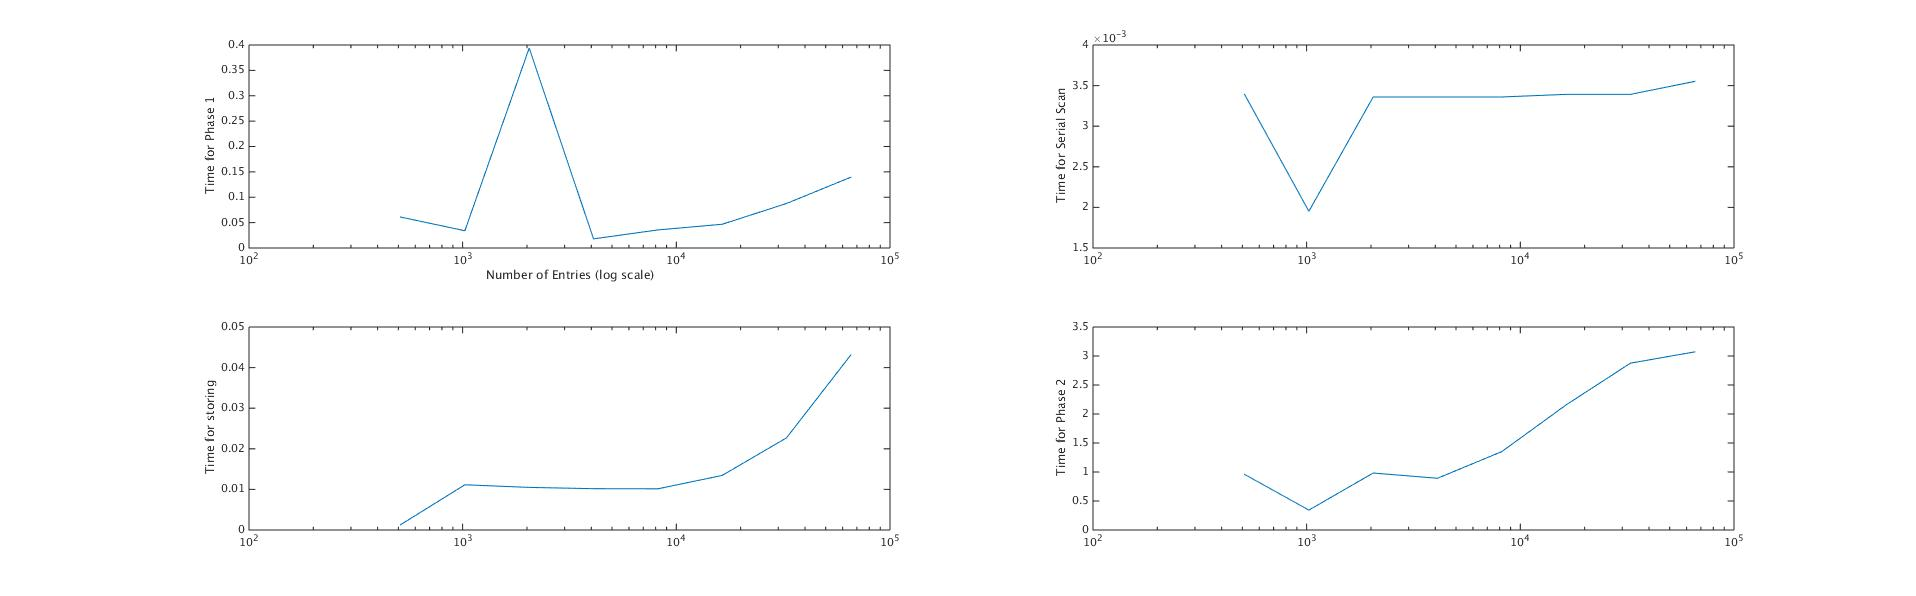
\includegraphics[scale=0.6,trim = 10cm 0 40cm 0]{allbuildtimes.jpg}\\
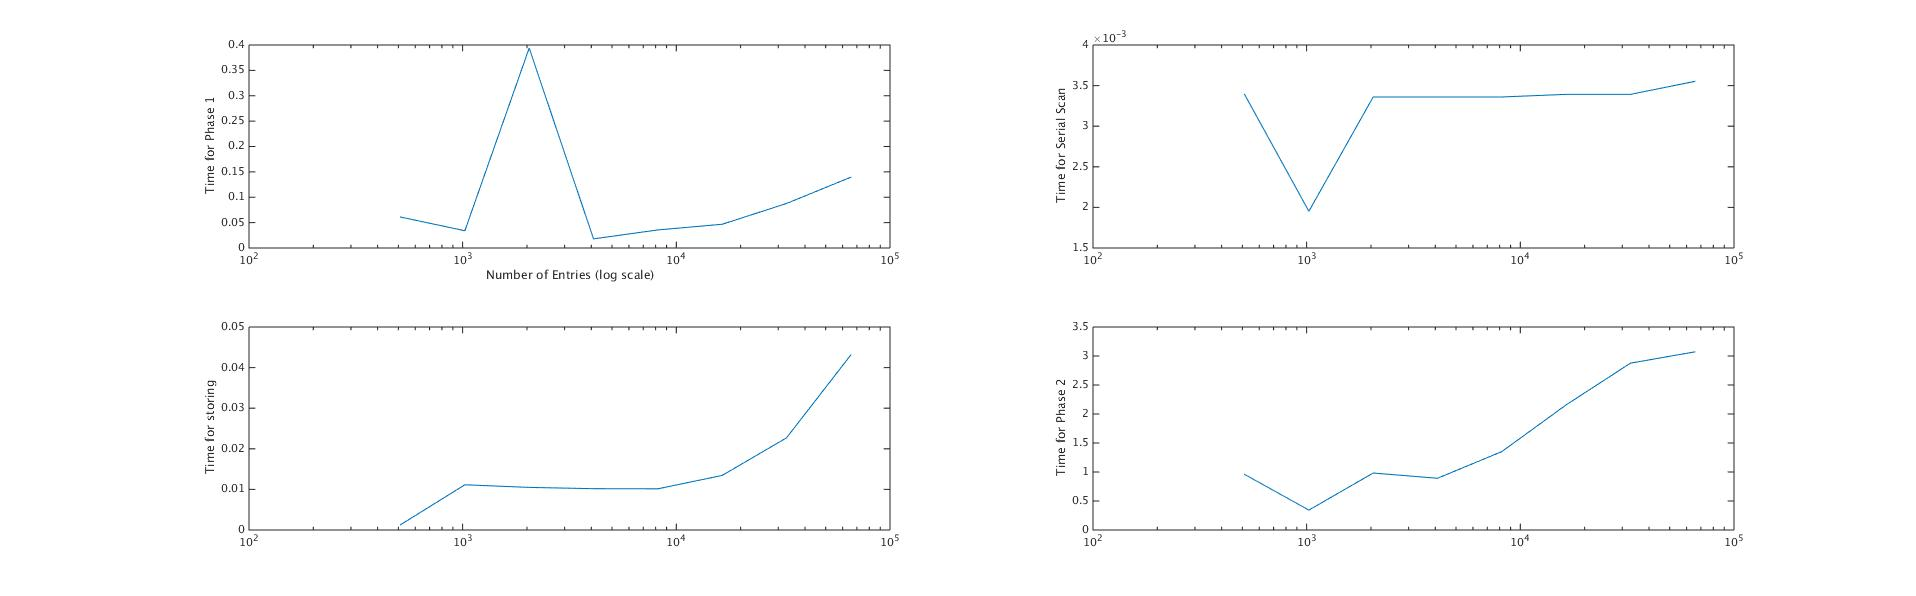
\includegraphics[scale=0.6,trim = 40cm 0 10cm 0 ]{allbuildtimes.jpg}
\label{all_lonestar}
\caption{Time for various kernels on Lonestar}
\end{figure}
\newpage
\begin{sidewaysfigure}
    \centering
    \begin{tikzpicture}[scale=1]
        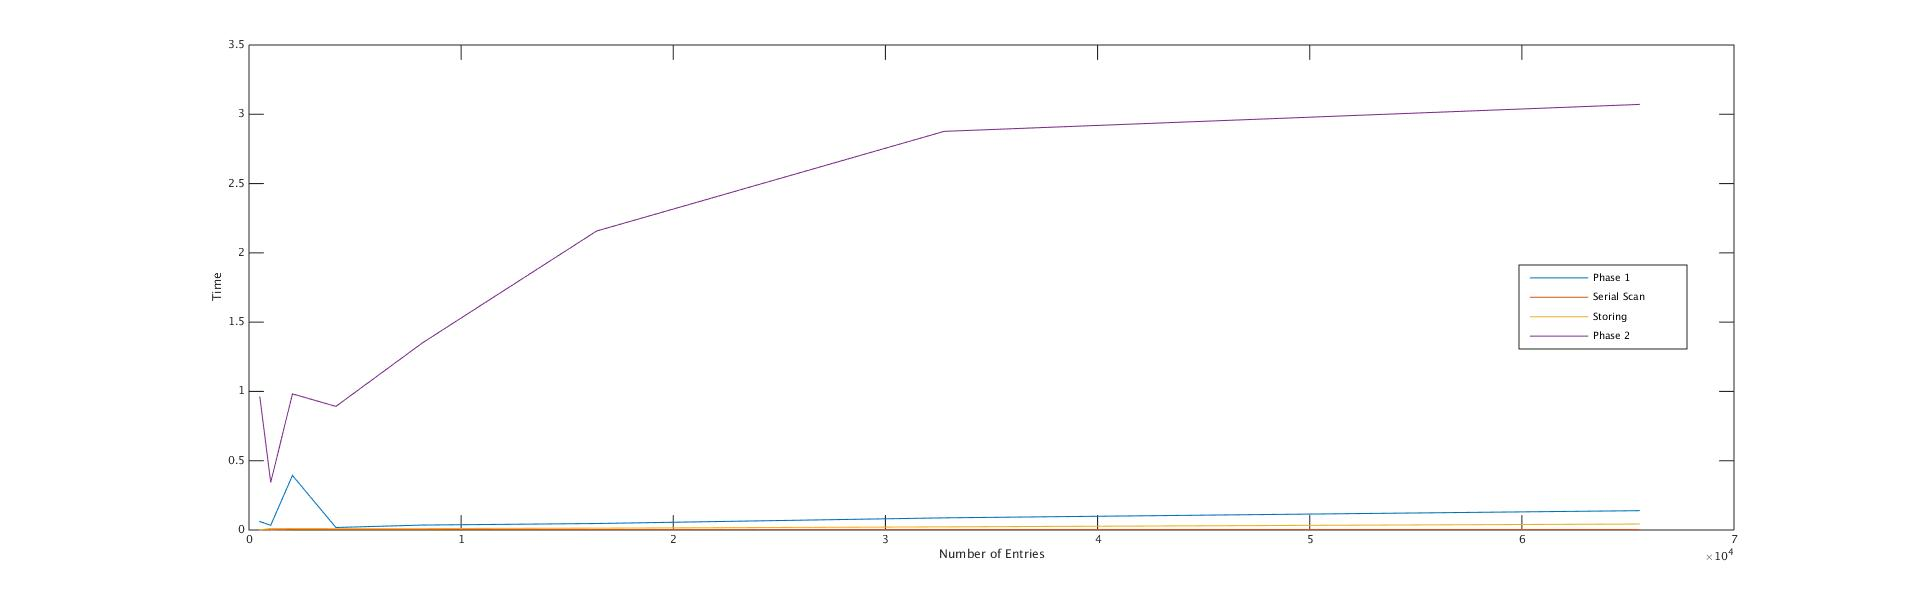
\includegraphics[scale=0.4, trim = 33cm 05cm 0 0]{allbuildtimesIn1.jpg}       
      \end{tikzpicture}
    \caption{Comparing time required by each kernel for lonestar}
    \label{fig:allin1ls}
\end{sidewaysfigure}
\begin{sidewaysfigure}
    \centering
    \begin{tikzpicture}[scale=1]
        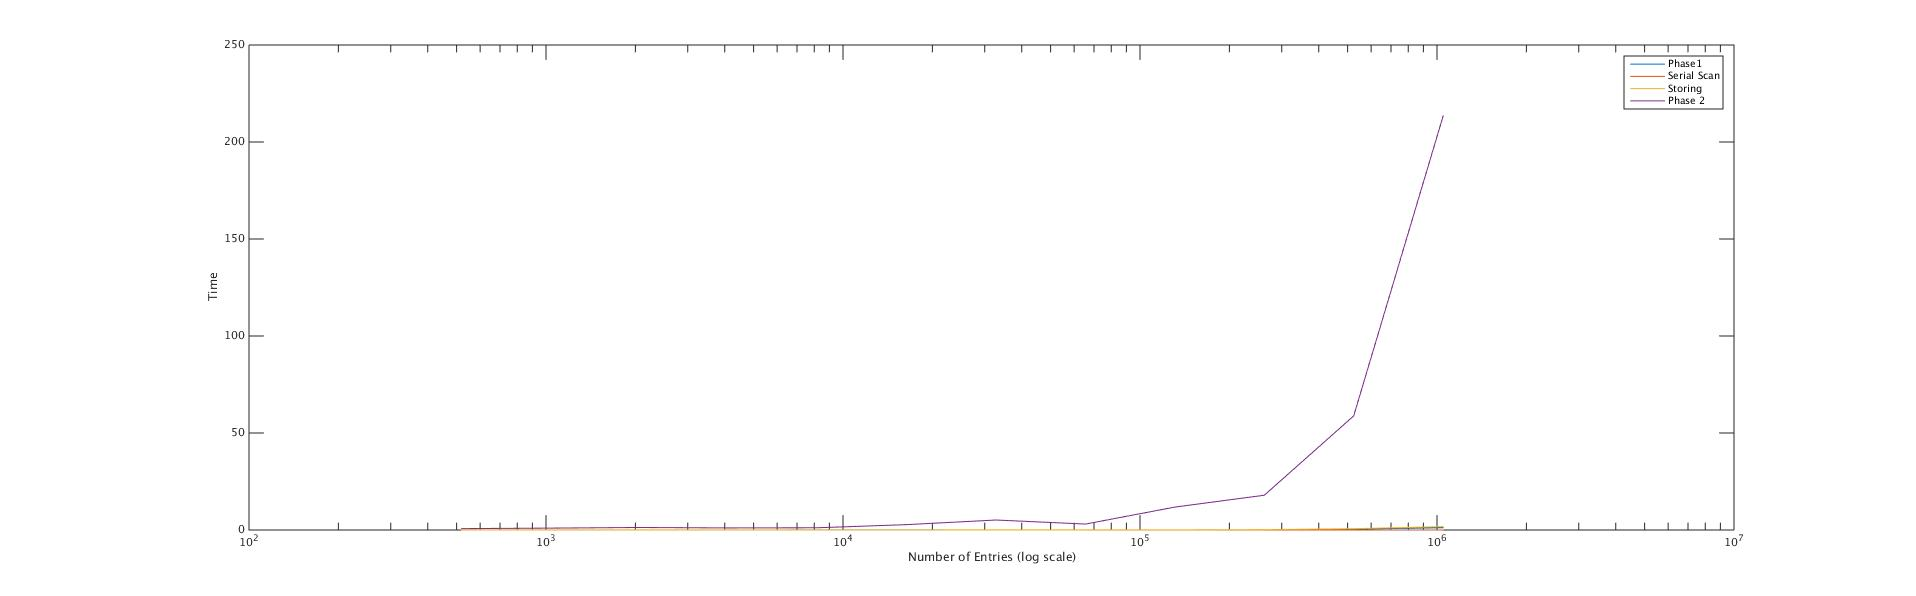
\includegraphics[scale=0.4, trim = 33cm 05cm 0 0]{allbuildtimesIn1_hardy.jpg}       
      \end{tikzpicture}
    \caption{Comparing time required by each kernel for hardy}
    \label{fig:allin1hd}
\end{sidewaysfigure}
\begin{thebibliography}{9}

\bibitem{1}
  Alcantara D.A.F.,
  \emph{Efficient Hash Tables on the GPU},
  University of California,Davis
  2011.
  
 \bibitem{2}
 CUDA C-Programming Guide- http://docs.nvidia.com/cuda/cuda-c-programming-guide/
\end{thebibliography}
\end{document}